\chapter{Reactive silicon dioxide}
\label{reactive-silicon-dioxide-label}

\vspace{-1cm} \noindent \textcolor{graytitle}{\textit{{\Large Simulating a chemically reactive structure}}\vspace{0.5cm} }

\noindent \hspace{-0.45cm}\begin{wrapfigure}{r}{4cm}
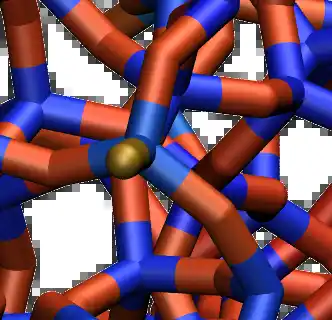
\includegraphics[width=4cm]{tutorials/level3/reactive-silicon-dioxide/SiO_gif_light.png}
\end{wrapfigure}

\noindent The objective of this tutorial is to use a molecular
dynamics system made of silicon dioxide (SiO2), and deform 
it until it breaks. The reactive force field \textit{reaxff} is used, and 
a particular attention is given to the evolution of the charges
of the atoms during the deformation of the structure. 

\section{Relax the structure}

\noindent Create a folder, name it RelaxSilica/, and \href{../../../../../inputs/level3/reactive-silicon-dioxide/RelaxSilica/silica.data}{download}
the initial topology of a small amorphous silica structure.
The system was created by temperature annealing using another force field 
(\href{../../../../../inputs/level3/reactive-silicon-dioxide/CreateSilica/SiO.1990.vashishta}{vashishta}), therefore the structure is slightly
different to what is expected from the reaxff force field. 
For instance, the average bond lengths, angles, and charges 
are likely to be different, and the structure needs 
to be relaxed again using reaxff. 
If you are interested, the input file used for creating the initial topology is 
available \href{../../../../../inputs/level3/reactive-silicon-dioxide/CreateSilica/input.lammps}{here}, but its description is not part of this tutorial.
The Atoms section of the \textit{silica.data} file starts like that:

\begin{lcverbatim}
Atoms # full
132 15 2 -0.55 1.722106654667303 6.0790786378597526 5.627968948336774 -6 4 -5
172 20 1 1.1 5.755393150671698 3.31535305846982 1.0501387543709164 4 3 2
231 26 2 -0.55 5.617126717910301 7.487471864752421 1.963810241571427 -16 8 -3
54 6 2 -0.55 4.060884959755418 1.6283060986470597 4.297860218329581 -7 -4 3
174 20 1 1.1 2.9926597997825395 2.0364512736354192 0.7520371846065788 -2 -6 -7
180 20 2 -0.55 3.18438907446254 2.5721052475107857 6.622363526485664 0 -12 1
121 14 2 -0.55 5.537222937373211 1.456250286791573 6.343752399466858 -9 -12 -4
111 13 1 1.1 1.7279273441891305 7.28674041911877 6.669158065545038 6 -10 -2
51 6 2 -0.55 5.366932941422638 4.1504125630630435 2.3740196532457105 0 -1 -3
202 23 2 -0.55 7.313845702241226 3.321272888336706 3.777618751313188 0 5 -13
215 24 2 -0.55 6.690317849940269 5.754543737004929 4.103252634559489 -6 2 0
183 21 1 1.1 1.777618482333677 6.145548171417662 3.999369841948803 -5 -5 -3
95 11 2 -0.55 4.561227581704491 2.3474960588346616 0.6330321107351076 -1 -6 3
105 12 2 -0.55 5.0710009155644125 3.8511969818510208 5.143556706337486 -1 0 5
(...)
\end{lcverbatim}

\noindent Due to the use of vashishta force field for creating the initial configuration,
all silicon atoms have the same charge q = 1.1e,
and all oxygen atoms the charge q = -0.55e. This is common to most
classical force field. Let us keep that in mind before we start using \textit{reaxff}.
The first step is to relax the structure, which we are gonna do using molecular
dynamics. To make sure that the system equilibrates nicely, let us track the
changes in our system over time. 
Create an input file called input.lammps in RelaxSilica/, and copy in it: 

\begin{lcverbatim}
units real
atom_style full
read_data silica.data
mass 1 28.0855 # Si
mass 2 15.999 # O
\end{lcverbatim}

\noindent So far, the input is very similar to what is seen in the other tutorials here,
with some basic parameters being defined (\textit{units}, \textit{atom$\_$style} and \textit{masses}), and 
the data file being imported by the \textit{read$\_$data} command.
Now let us enter 3 crucial lines:

\begin{lcverbatim}
pair_style reaxff NULL safezone 3.0 mincap 150
pair_coeff * * reaxCHOFe.ff Si O
fix myqeq all qeq/reaxff 1 0.0 10.0 1.0e-6 reaxff maxiter 400
\end{lcverbatim}

\noindent Here, the reaxff \textit{pair$\_$style} is used with no control file, and the \textit{safezone} and \textit{mincap}
keywords have been added for memory allocation issue. If not there, the segmentation
faults and bondchk failed errors sometimes occur.
The \textit{pair$\_$coeff} uses the \href{../../../../../inputs/level3/reactive-silicon-dioxide/RelaxSilica/reaxCHOFe.ff}{reaxCHOFe.ff} file which is assumed to be saved in the
same folder as the input. The atoms of type 1 are set as silicon (Si),
and type 2 as oxygen (O) in order to be consistent with the data file and
mass definition.
Finally, the fix \textit{qeq/reaxff} is used to perform charge equilibration every timestep. The values 0 and 10.0
are low and high cutoffs, respectively, and $1.0 \text{e}-6$ a tolerance. Finally, maxiter sets
a limit to the number of attempt to equilibrate the charge. 

\begin{tcolorbox}[colback=mylightblue!5!white,colframe=mylightblue!75!black,title=Note]
If the charge does not
properly equilibrate despite the 400 attempts, a warning will appear. Such warning
are likely to appear if the initial charges are too far from equilibrium values. 
\end{tcolorbox}

\noindent Then, let us use some (familiar) commands controlling the building of the 
neighbor lists. Let us also print thermodynamic information, the charge of both atom types,
and create a dump file for visualization.

\begin{lcverbatim}
neighbor 0.5 bin
neigh_modify every 5 delay 0 check yes 
group grpSi type 1
group grpO type 2
variable totqSi equal charge(grpSi)
variable totqO equal charge(grpO)
variable nSi equal count(grpSi)
variable nO equal count(grpO)
variable qSi equal v_totqSi/${nSi}
variable qO equal v_totqO/${nO}
dump dmp all custom 100 dump.lammpstrj id type q x y z
thermo 10
thermo_style custom step temp etotal press vol v_qSi v_qO
\end{lcverbatim}

\noindent Let us perform a very short run using anisotropic NPT command
and relax the density of the system. 

\begin{lcverbatim}
velocity all create 300.0 3482028
fix mynpt all npt temp 300.0 300.0 10 aniso 1.0 1.0 100
timestep 0.5
run 2000
\end{lcverbatim}

\noindent \begin{tcolorbox}[colback=mylightblue!5!white,colframe=mylightblue!75!black,title=Note]
Here, I choose values of 10 fs for the temperature damping parameter and 100 fs
for the pressure. These choices were made to reach equilibrium faster and 
allow very short run to be performed. For an actual simulation (and not a tutorial),
longer equilibration and larger damping times should be used (100 fs and 1000 fs
for temperature and pressure respectively are usually used for atomic systems).
\end{tcolorbox}

\noindent As the simulation runs, you can see that the charges of the atoms are fluctuating,
as the atoms adjust themselves to the topology:

\begin{figure}
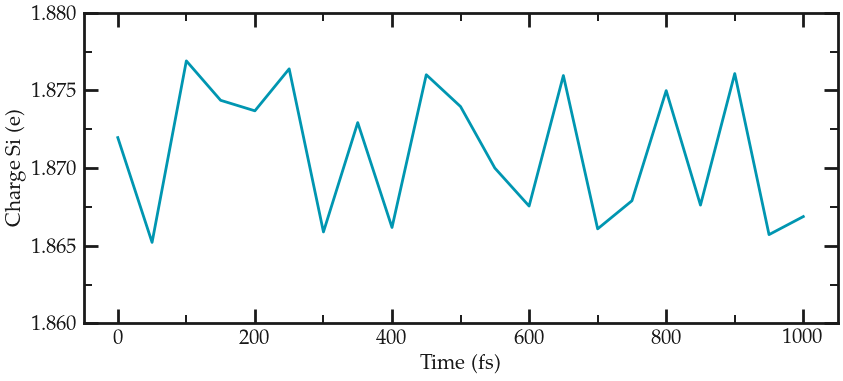
\includegraphics[width=\linewidth]{tutorials/level3/reactive-silicon-dioxide/average-charge-light.png}
\end{figure}

Moreover, and because each atom adopts its own fluctuating charge value,
the charges are distributed around a mean value:

\begin{figure}
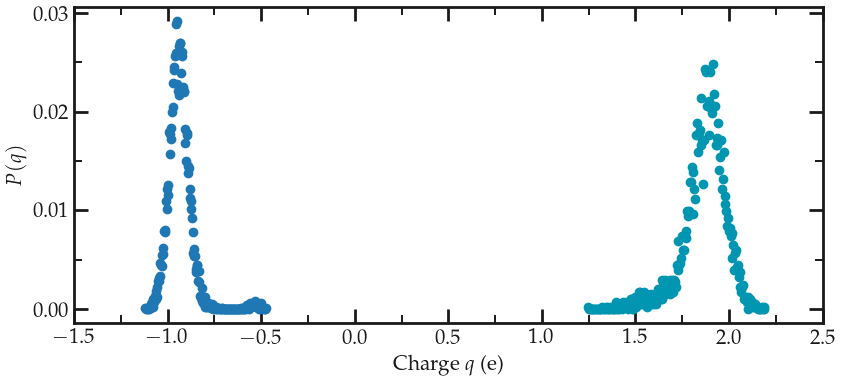
\includegraphics[width=\linewidth]{tutorials/level3/reactive-silicon-dioxide/distribution-charge-light.png}
\end{figure}

Using VMD and coloring the atoms by their charges, one can see that 
the atoms with the extreme-most charges are located at defects in the 
amorphous structure (here at the positions of the dandling oxygen groups):

\begin{figure}
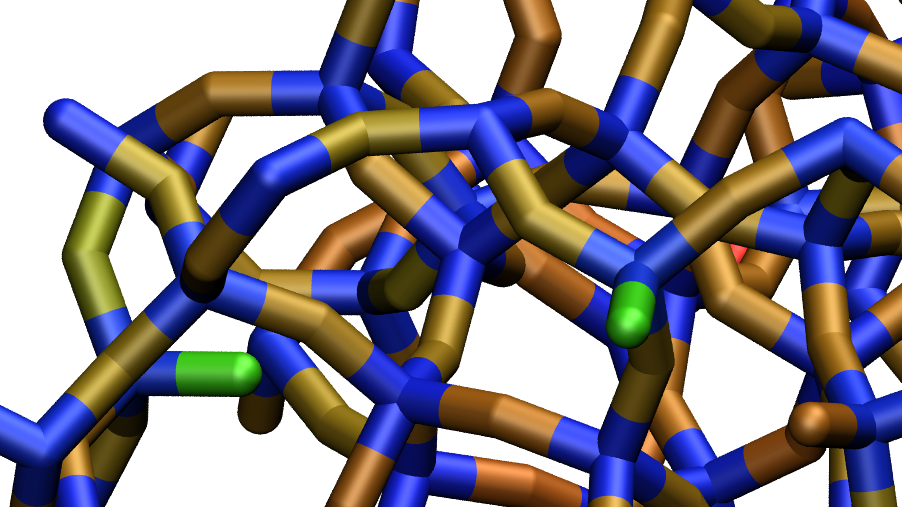
\includegraphics[width=\linewidth]{tutorials/level3/reactive-silicon-dioxide/silicon-light.png}
\end{figure}

Note for VMD user: to color the atoms by their charge, use \textit{Charge} as coloring method in the 
representation windows, and then tune the \textit{Color scale} in the \textit{Color control windows}.

\section{Deform the structure}

\noindent Let us apply a deformation to the structure in order to force some bonds 
to dynamically break and reassemble. 
Next to \textit{RelaxSilica/}, create a folder, call it \textit{Deform/} and create a
file named input.lammps in it. Copy the following lines:

\begin{lcverbatim}
# SiO amorphous silica deformed with reaxff potential
units real
atom_style full
read_data ../RelaxSilica/silica-relaxed.data
mass 1 28.0855 # Si
mass 2 15.999 # O
pair_style reaxff NULL safezone 3.0 mincap 150
pair_coeff * * ../RelaxSilica/reaxCHOFe.ff Si O
fix myqeq all qeq/reaxff 1 0.0 10.0 1.0e-6 reaxff maxiter 400
neighbor 0.5 bin
neigh_modify every 5 delay 0 check yes 
group grpSi type 1
group grpO type 2
variable totqSi equal charge(grpSi)
variable totqO equal charge(grpO)
variable nSi equal count(grpSi)
variable nO equal count(grpO)
variable qSi equal v_totqSi/${nSi}
variable qO equal v_totqO/${nO}
dump dmp all custom 100 dump-deform.lammpstrj id type q x y z
thermo 100
thermo_style custom step temp etotal press vol v_qSi v_qO
fix mynvt all nvt temp 300.0 300.0 100
timestep 0.5 
run 2000
fix mydef all deform 1 x erate 5e-5
run 25000
unfix mydef
undump dmp
dump dmp all custom 100 dump.lammpstrj id type q x y z
run 2000
write_data silica-deformed.data
\end{lcverbatim}

\noindent The main differences with the previous input are
\begin{itemize}
\item the use of fix deform for elongating progressively the box along x,
\item the use of fix NVT instead of NPT (because the box deformation is already ensured by fix deform).
\end{itemize}

After a first run of 25000 steps, a short run of 2000 steps is performed 
in order to extract the final charges of the atoms from an structure that is not 
under deformation.
During the deformation, the charges progressively changes, until the structure eventually
breaks up. After the structure breaks, the charges equilibrates near a new 
average value that differs from the starting charge, which is expected due to the
presence of the new solid/vacuum interface:

\begin{figure}
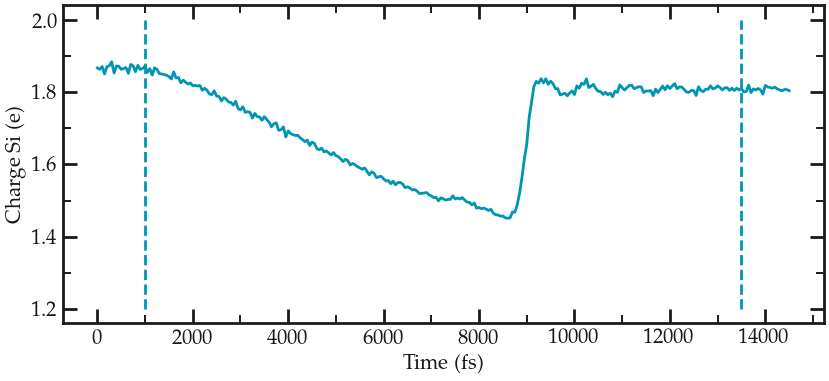
\includegraphics[width=\linewidth]{tutorials/level3/reactive-silicon-dioxide/deformed-charge-light.png}
\end{figure}

At the end of the deformation,  one can visualize the broken material. Notice
the different charge of the atoms located near the interface and compared to the 
atoms located in the bulk of the material:

\begin{figure}
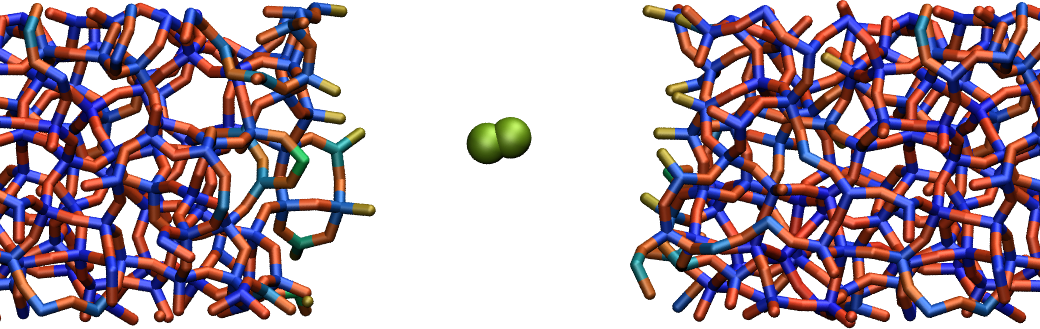
\includegraphics[width=\linewidth]{tutorials/level3/reactive-silicon-dioxide/deformed-light.png}
\end{figure}

One O2 molecule was formed during the process (here appearing in green),
most likely because the rate of deformation was really high.
One can have a look at the final charge distribution:

\begin{figure}
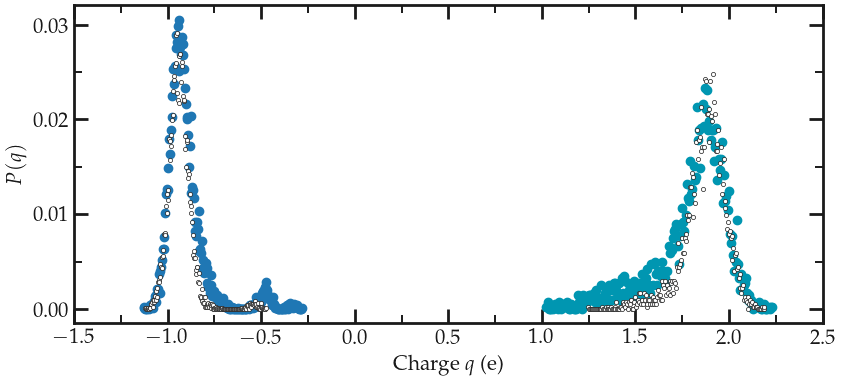
\includegraphics[width=\linewidth]{tutorials/level3/reactive-silicon-dioxide/deformed-distribution-charge-light.png}
\end{figure}

The final charge distribution differs from the previously calculated, as a new peak 
near -0.5e for the oxygen. 

\section{Add O2 molecules}

\noindent Let us add more O2 molecule to our previously equilibrated structure, equilibrate it again, 
and extract the charge density profile along the x axis.
Create a new folder, name it AddOxygen/, and create a new molecule file named O2.mol in it:

\begin{lcverbatim}
# O2 reaxff file
2 atoms
Coords
1 -0.6 0 0
2 0.6 0 0
Types
1        2
2        2   
Charges 
1	0.0
2	0.0
\end{lcverbatim}

\noindent Here the O2 molecule is simply made of 2 oxygen (type 2) atoms that are not 
connected by any bond (because there is no need with reaxff).
Then, create a new input.lammps file, and copy the same first lines as
previously in it: 

\begin{lcverbatim}
units real
atom_style full
read_data ../Deform/silica-deformed.data
mass 1 28.0855 # Si
mass 2 15.999 # O
pair_style reaxff NULL safezone 3.0 mincap 150
pair_coeff * * ../RelaxSilica/reaxCHOFe.ff Si O
fix myqeq all qeq/reaxff 1 0.0 10.0 1.0e-6 reaxff maxiter 400
neighbor 0.5 bin
neigh_modify every 5 delay 0 check yes 
\end{lcverbatim}

\noindent Optionally, let us shift the structure to recenter it in the box. The best value 
for the shift may be different in your case. This step is not necessary, but the
recentered system looks better.

\begin{lcverbatim}
displace_atoms all move -13 0 0 units box
\end{lcverbatim}

\noindent Then, let us import the molecule template O2.mol and create 10 molecules. 
The overlap and maxtry keywords allow us to prevent overlapping
between the atoms:

\begin{lcverbatim}
molecule O2mol O2.mol
create_atoms 0 random 10 456415 NULL mol O2mol 454756 overlap 3.0 maxtry 50
\end{lcverbatim}

\noindent The value of 3 Angstroms for the minimum interatomic overlapping is 
very safe for the present system. Smaller values may lead to molecules being 
too close from each others.
Finally, let us minimize the energy of the system, and run for a relatively long time:

\begin{lcverbatim}
minimize 1.0e-4 1.0e-6 100 1000
reset_timestep 0
group grpSi type 1
group grpO type 2
variable totqSi equal charge(grpSi)
variable totqO equal charge(grpO)
variable nSi equal count(grpSi)
variable nO equal count(grpO)
variable qSi equal v_totqSi/${nSi}
variable qO equal v_totqO/${nO}
dump dmp all custom 1000 dump.lammpstrj id type q x y z
thermo 1000
thermo_style custom step temp etotal press vol v_qSi v_qO
fix mynvt all nvt temp 300.0 300.0 100
timestep 0.5 
run 100000
\end{lcverbatim}

\noindent Run the simulation. You should see additional O2 molecules in the system:

\begin{figure}
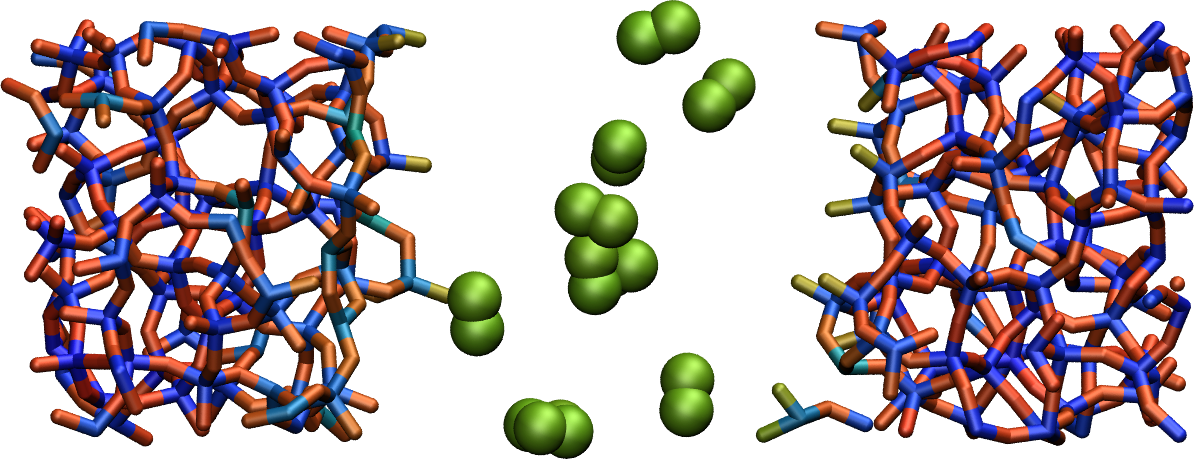
\includegraphics[width=\linewidth]{tutorials/level3/reactive-silicon-dioxide/O2_light.png}
\end{figure}

\section{Exercises}

\noindent \subsection{Decorate dandling oxygens}

Under ambient conditions, dandling oxygen are typically terminated by hydrogen atoms. 
Let us improve the current structure by decorating some of the dandling oxygen with
hydrogen atoms, before relaxing it thanks to reaxff. 
Add hydrogen atoms to the dandling oxygens. Then relax the structure using \textit{reaxff} with LAMMPS.
Hydrogen atoms can be added using \textit{create$\_$atoms} command, \textit{gcmc}, or external \textit{Python} script as I did here:

\begin{figure}
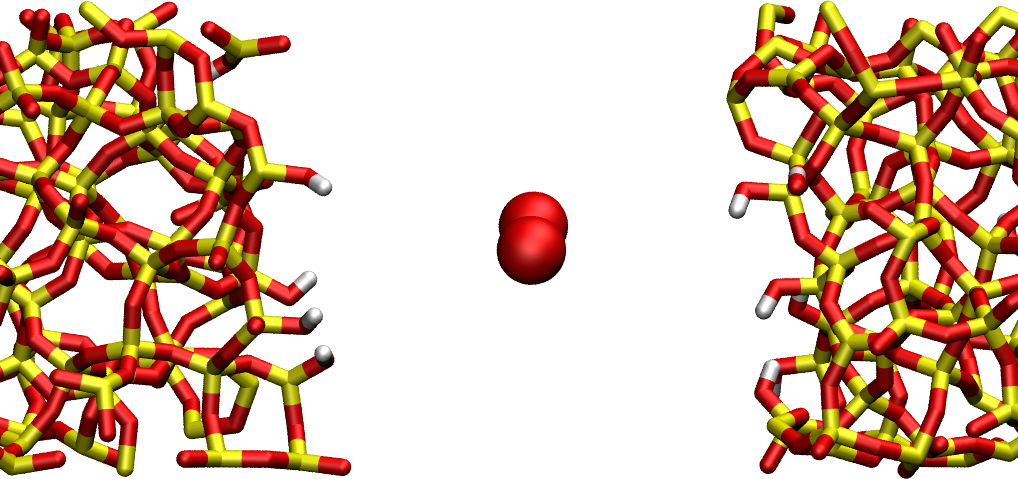
\includegraphics[width=\linewidth]{tutorials/level3/reactive-silicon-dioxide/exercice-light.png}
\end{figure}

\begin{tcolorbox}[colback=mylightblue!5!white,colframe=mylightblue!75!black,title=Hint n°1]
The structure can be imported in MDAnalysis/Python using \textit{u = mda.Universe("silica-deformed.data")}
Then dandling oxygen can be detected by counting the number of neighbor (oxygen with only 
one connected silicon is dandling and should be completed with an hydrogen).
\end{tcolorbox}

\noindent \begin{tcolorbox}[colback=mylightblue!5!white,colframe=mylightblue!75!black,title=Hint n°2]
Once hydrogen have been added, run LAMMPS using:
\begin{lcverbatim}
mass 1 28.0855 # Si
mass 2 15.999 # O
mass 3 1.008 # H
\end{lcverbatim}

\noindent and:
\begin{lcverbatim}
pair_coeff * * reaxCHOFe.ff Si O H
\end{lcverbatim}

\noindent \end{tcolorbox}

